
\documentclass{article} % For LaTeX2e
\usepackage{iclr2026_conference,times, graphicx, float, hyperref}
\iclrfinalcopy

% Optional math commands from https://github.com/goodfeli/dlbook_notation.
\input{math_commands.tex}

\usepackage{hyperref}
\usepackage{url}


\title{AI Based Vanity License Plate Discovery}

% Authors must not appear in the submitted version. They should be hidden
% as long as the \iclrfinalcopy macro remains commented out below.
% Non-anonymous submissions will be rejected without review.

\author{Daniel Lobenstein \\
Department of Electrical- and Computer Engineering\\
Purdue University\\
Schopfheim, Baden-Württemberg 79650, Germany \\
\texttt{dlobenst@purdue.edu} 
}

% The \author macro works with any number of authors. There are two commands
% used to separate the names and addresses of multiple authors: \And and \AND.
%
% Using \And between authors leaves it to \LaTeX{} to determine where to break
% the lines. Using \AND forces a linebreak at that point. So, if \LaTeX{}
% puts 3 of 4 authors names on the first line, and the last on the second
% line, try using \AND instead of \And before the third author name.

\newcommand{\fix}{\marginpar{FIX}}
\newcommand{\new}{\marginpar{NEW}}

%\iclrfinalcopy % Uncomment for camera-ready version, but NOT for submission.
\begin{document}


\maketitle

\begin{abstract}
The procurement of vanity license plates represents a highly sought-after personalization service and a notable revenue stream for state agencies. However, existing discovery systems rely on a highly manual, high-friction "guess-and-check" paradigm, leading to frustrating user experiences and diminished conversion rates. While current third-party tools can generate ideas, they fail to deterministically verify real-time availability against state registries. To address this bottleneck, this paper introduces a novel AI-driven recommendation architecture that bridges stochastic Large Language Model (LLM) text generation with deterministic state-registry verification. The proposed framework features a closed-loop iterative pipeline that translates semantic user inputs into format-compliant candidate strings, checks their availability, and autonomously utilizes negative feedback to refine subsequent generations until a target quota of available plates is successfully curated. A functional Proof of Concept (PoC) was developed utilizing a decoupled client-server architecture, demonstrating the technical feasibility of the system. Qualitative evaluation through stakeholder engagement—including discussions with leadership at the California Department of Motor Vehicles (DMV)—validated the framework's core advantages and potential value. While direct deployment faces institutional data-access constraints, the prototype successfully establishes a scalable, automated foundation for modernizing public sector administrative interfaces and maximizing state revenue opportunities.
\newline
\href{https://github.com/lobendan/ai_project}{Code and Latex}
\end{abstract}

\section{Introduction}

The procurement of customized vehicle registration identifiers—commonly referred to as vanity license plates—constitutes a highly sought-after personalization service for citizens and a notable revenue stream for state agencies. However, while recent advancements in Generative Artificial Intelligence, specifically Large Language Models (LLMs), have demonstrated profound capabilities in ideation and natural language processing, their application in constrained administrative environments remains underutilized.\cite{ai_public_sector} Existing consumer solutions, in this specific field, often decouple the creative generation of ideas from the deterministic validation of those ideas against real-world regulatory constraints. To mitigate systemic bottlenecks in the public sector, this paper introduces a novel, AI-driven vanity plate recommendation architecture designed to synthesize stochastic text generation with deterministic state-registry verification.

\subsection{Problem Statement}

The existing infrastructure for discovering available vanity license plates is fundamentally constrained by an inefficient search paradigm. The current process dictates a frustrating user experience that is inherently manual and highly repetitive. Users are subjected to high friction, as they must enter each plate idea individually and manually trigger an availability check for every single attempt. Furthermore, because most desirable combinations are already taken in many states, users frequently encounter a "dead-end" experience characterized by a low success rate, where search queries repeatedly return as "unavailable." Ultimately, this systemic inefficiency and poor user experience directly result in lower conversion rates, precipitating significant missed revenue opportunities for state agencies.

\begin{figure}[htbp]
    \centering
    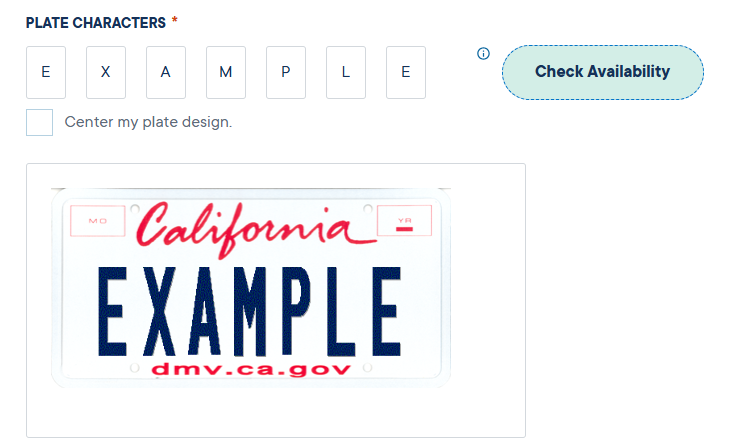
\includegraphics[width=0.6\linewidth]{dmv_example.png}
    \caption{The California DMV's current vanity license plate discovery system, which relies on a manual query process.}
    \label{fig:CaliDMVExample}
\end{figure}

As illustrated in Figure \ref{fig:CaliDMVExample}, the current vanity license plate discovery system of the California DMV requires users to manually input a concept and subsequently press the "Check Availability" button. The system then takes several seconds to return a result. Should the user wish to query another idea, they must manually delete the previous input, enter the new string, and re-initiate the availability check. For users attempting to secure a desirable and available vanity plate, this process necessitates numerous iterations. It quickly becomes frustrating and frequently leads to user abandonment. While this specific example highlights the California system, interfaces in other U.S. states demand a similar degree of manual effort. 

\subsection{Intended Solution}

To resolve these critical bottlenecks, the proposed framework introduces a goal-oriented system capable of delivering AI-driven plate recommendations. The architecture transitions the user interface from a manual, iterative search to one utilizing natural language input, enabling users to simply prompt the system with personal information or thematic elements related to their desired plate.

This semantic input is processed by an AI-powered generation backend that creates highly tailored vanity plate ideas. Crucially, the final framework will achieve proactive availability matching by routing these generated candidates through an availability engine, which verifies their real-time status.

A core innovation of this architecture is its dynamic feedback mechanism. Should the availability of an initial batch be low, the system's retry logic autonomously requests a new set of ideas from the LLM. During this loop, the system dynamically lowers a "rarity index" parameter and feeds back an exclusion list of previously checked, unavailable plates to prevent duplicate generation. The process loops continuously until the target count of verified-available plates is successfully curated, thereby providing the user with multiple tailored options that are guaranteed to be available in their respective state.

Implementing this solution inherently requires access to state-level vanity plate availability data. Currently, this data is not publicly accessible on a large scale outside of the aforementioned manual interfaces; no public vanity plate availability API could be identified for any U.S. state. Consequently, officials at various state DMVs and analogous institutions were contacted to discuss potential partnerships and data access. Through this outreach, contact was established with the Chief Digital Transformation Officer of the California DMV, Ajay Gupta \cite{CaliDMVLeadership}. Subsequent discussions yielded valuable insights regarding internal systems, some of which inform the context of this paper.

\section{Related Work}

As previously described, no US state currently employs a system that advances beyond manual entry and a trial-and-error approach. Several external tools exist that generate vanity plate ideas, such as \textit{getmylp.com} and \textit{tagyourride.com}, alongside similar mobile applications. The critical limitation of these tools is that they exclusively generate ideas without verifying actual availability. While helpful for brainstorming, this still necessitates manual verification against state databases, which rapidly leads to frustration if many of the suggested ideas are already claimed. 

During the aforementioned discussions with state leadership, Mr. Gupta described a legacy system previously utilized by the state that provided users with available suggestions similar to their queried idea. This system is no longer in use. It is important to note that this prior attempt operated with significantly less context regarding user preferences, as the sole input was the single string the user attempted to check. In the proposed solution, the LLM leverages a substantially broader context provided by the user's prompt to generate highly relevant and personalized plate candidates.

\section{Methodology}

The methodology of this research employs a decoupled, highly scalable client-server architecture to facilitate AI-driven vanity license plate discovery. The core computational backend is encapsulated as an asynchronous REST API utilizing the FastAPI framework. This endpoint leverages a Large Language Model (LLM) equipped with optimized prompt engineering to iteratively generate contextually relevant, format-compliant candidate strings based on semantic user inputs. To ensure jurisdictional compliance, the generative process is governed by a centralized, parameterized configuration module that dynamically enforces state-specific heuristic constraints—such as strict alphanumeric length boundaries, rarity indexing, and algorithmic retry limits—while remaining abstracted from the end user. 

Incoming API requests are strictly validated using Pydantic data models before processing. Furthermore, to maximize time and computational resource efficiency during the development phase, the live web-scraping verification engine was superseded by a stochastic simulation environment. This emulator utilizes probabilistic randomization to approximate real-time database availability queries, acting as a modular proxy for future direct DMV API integrations. Finally, this backend infrastructure interfaces via secure tunneling (ngrok) with a functional frontend prototype engineered on the Retool platform, enabling seamless, end-to-end evaluation of the generative pipeline.

\section{Implementation}

\subsection{System Architecture}

\begin{figure}[htbp]
    \centering
    
\includegraphics[width=0.75\linewidth]{iclr2026/AIPlateGetter.drawio.png}
    \caption{Sequence Diagram of the AI-driven recommendation architecture.}
    \label{fig:SeqDiagram}
\end{figure}

The implementation follows the sequence shown in Figure \ref{fig:SeqDiagram} as a service-orchestrated pipeline centered on the API layer. A user request enters through the UI as \texttt{POST /find-plates}, after which the API server executes an iterative control loop that continues until either the target number of available vanity plates is reached or a configured retry bound is met. Within each iteration, the server invokes \texttt{generate\_plate\_ideas()} against the LLM API (currently \texttt{gemini-2.5-flash} is used) to produce a batch of candidate strings conditioned on user intent and constraint settings. It then forwards that batch to the plate-availability interface (\texttt{check\_plates()}), representing the DMV availability endpoint in the architecture. 

The checker response is partitioned into available and unavailable sets, and both are persisted in the loop state so subsequent LLM calls can exploit negative feedback (unavailable history) to reduce the regeneration of previously rejected candidates and improve convergence efficiency. This closed-loop design separates generation from validation while preserving clear system boundaries: creative synthesis is delegated to the LLM service, authoritative feasibility is delegated to the external availability service, and policy/governance logic (termination, batching, and filtering) remains in the API orchestration layer. The final response returned to the UI is a typed \texttt{List<AvailablePlates>}, yielding a deterministic API contract despite the stochastic candidate generation inside the loop.

\subsection{Prototype User Interface}

\begin{figure}[htbp]
    \centering
    
\includegraphics[width=0.65\linewidth]{iclr2026/demo_gui_example.png}
    \caption{Frontend prototype graphical user interface for natural language plate discovery.}
    \label{fig:GUI}
\end{figure}

Figure \ref{fig:GUI} demonstrates a functional prototype of the improved system. The interface allows the user to adjust the length range of the plate ideas, specify the desired quantity of suggestions, and enter a natural language prompt to describe the thematic context of the plates they wish to receive. Upon clicking the "Find Plates" button, the system calls the REST API and subsequently displays a curated list of available vanity plates matching the given prompt. This demonstration is powered by Retool and connected to the REST API endpoint utilizing ngrok.

\section{Evaluation}

The primary evaluation objective for this phase was to establish a Proof of Concept (PoC). The successful implementation of the initial prototype demonstrates the technical feasibility and core advantages of the proposed system over existing alternatives. Furthermore, the prototype served as an effective demonstration tool during a presentation with a potential state partner, yielding positive qualitative feedback and validating the underlying concept. 

During this meeting, it became evident that obtaining external access to internal APIs—such as the one required for real-time availability checks—is currently unfeasible for an outside entity interacting with the California DMV. However, the conceptual progress remains of significant interest to the California DMV, and potential collaborations between the agency and the author, or Purdue University more broadly, are actively being discussed at the time of writing.

\section{Conclusion}

This paper presented a novel, AI-driven framework designed to resolve the systemic inefficiencies inherent in current vanity license plate discovery processes. By transitioning the user interface from a manual, high-friction search paradigm to a semantic, goal-oriented recommendation system, the proposed architecture significantly enhances the user experience while presenting state agencies with an opportunity to recover missed revenue streams. The successful implementation of a functional Proof of Concept (PoC) validated the core methodology: coupling the creative, stochastic generation capabilities of Large Language Models with a deterministic validation loop. This iterative orchestration effectively filters unavailable candidates and autonomously refines generation, ensuring users are solely presented with viable, available options tailored to their prompt.

Qualitative evaluation of the prototype yielded positive feedback, particularly during a stakeholder discussion with the California DMV. However, this research also highlighted a critical practical limitation: the strict institutional barriers preventing external access to real-time, large-scale DMV availability databases. Consequently, while the current backend relies on a stochastic simulation environment for verification, the logical next step for this research is achieving real-world integration. Future work will focus on advancing ongoing collaboration discussions between academic institutions, such as Purdue University, and state entities to establish secure, compliant API access to live registry data. Ultimately, this research provides a highly scalable blueprint for leveraging generative AI to streamline and modernize constrained administrative environments in the public sector.



\subsubsection*{LLM Acknowledgment}
An LLM was used to improve the text and formatting of this paper. Following prompt has been used: "Improve this text and formatting, without changing its content. It shall follow ICLR formatting, give me the raw Latex code."


\bibliography{iclr2026_conference}
\bibliographystyle{iclr2026_conference}



\end{document}
